\section{Software-Entwurf mit FSM}
\subsection{Aufgabenstellung}
\begin{enumerate}%Aufzählung mit Numerierung
		\item Entprellen der Taster
		\begin{itemize}
			\item Messen Sie die typische Prelldauer einer Taste mit dem Oszilloskop. Welche Entprellzeit schlagen Sie vor?
			\item Schreibe Sie eine Funktion \texttt{isPressed()}, mit der Tasteneingaben entprellt werden. 
		\end{itemize}
		\item LED mit einem Taster an- und ausschalten
		\begin{itemize}
			\item Eine LED soll mit einem Tastendruck angeschaltet und mit einem weiteren Tastendruck ausgeschaltet werden.
			\item Optional: Mit jedem Tastendruck soll eine LED aus- und die nächste angeschaltet werden.
		\end{itemize}
		\item Nachbildung eines Treppenlichtautomaten
		\begin{itemize}
			\item Auf Tastendruck geht das Licht (LED) an
			\item Das Licht bleibt für eine bestimmte (tbd.) Zeit an
			\item Anschließend wird das Licht kontinuierlich bis auf Null gedimmt
			\item Der Automat soll nachtriggerbar sein
		\end{itemize}
\end{enumerate}
Hinweise zur Implementierung:
\begin{itemize}
	\item Modellieren Sie die Funktionalität als FSM (Moore-Automat).
	\item Beachten Sie, dass das Debouncen (Entprellen) bei beiden Flankenwechseln stattfinden muss
\end{itemize}

\subsection{Lösung}
\begin{enumerate}
		\item Es wurden mehrere Prellvorgänge mit dem Oszilloskop gemessen. Je nach verwendetem Taster und der Art wie man den Taster drückt sind verschiedenen Prellvorgänge aufgenommen worden, diese sind in Abbildung \ref{image:prellen} dargestellt.\newline
		Die längste aufgenommene Prelldauer beträgt 250us. Ich wähle jedoch pauschal eine Entprelldauer (\grqq Debounce-Time\grqq) von $1ms$ vor, da durch vorherige Programmierschritte festgelegt wurde, dass der Mikrocontroller die \grqq Loop\grqq zyklisch im Takt von $1ms$ durchläuft.\newline
		Die Funktion \textit{isPressedSW0()} (Listening \ref{lst:ispressedsw0}) wurde als Zustandsautomat Implementiert. Die Funktion sollte zyklisch aufgerufen werden. Eine Skizze des Zustandsautomats ist in Abbildung \ref{image:statemachineispressed} zu sehen.
		\item Es wurde eine Funktion geschrieben, welche immer bei einem Tastendruck (Flanke von High auf Low) die LED toggled (Listening \ref{lst:FlipFlopLED0}).
		\item Der Treppenlichtautomat wurde ebenfalls als Zustandsautomat implementiert, von der Auflistung des Quellcodes wird aus Übersichtsgründen abgesehen.
\end{enumerate}



\begin{lstlisting}[frame=htrbl, caption={Funktion isPressedSW0()}, label={lst:ispressedsw0}]
#define STATE_STABLE_HIGH   0
#define STATE_INSTABLE_HIGH 1
#define STATE_STABLE_LOW    2
#define STATE_INSTABLE_LOW  3
const uint16_t cui16DebounceTime=1;


uint8_t isPressedSW0()
{
	static uint8_t ui8State = STATE_STABLE_HIGH; //default state
	static uint16_t ui16Counter=0;
	uint8_t ui8ReturnValue=1;
	
	switch(ui8State)
	{             
	case STATE_STABLE_HIGH:
		if(digitalRead(SW0)==LOW)
		{
			ui8State = STATE_INSTABLE_HIGH;
			ui16Counter=0;
		}
		ui8ReturnValue= HIGH;
	break;
	
	case STATE_INSTABLE_HIGH:
		ui16Counter++;
		if(digitalRead(SW0)==LOW)
		{
			if( ui16Counter>=cui16DebounceTime )
			{
				ui8State = STATE_STABLE_LOW;
				ui8ReturnValue= LOW;
			}
			else
				ui8ReturnValue= HIGH;
		}
		else
		{
			ui8State = STATE_STABLE_HIGH;
			ui8ReturnValue= HIGH;
		}
	break;
	
	case STATE_STABLE_LOW:
		if(digitalRead(SW0)==HIGH)
		{
			ui8State = STATE_INSTABLE_LOW;
			ui16Counter=0;
		}
		ui8ReturnValue= LOW;
	break;
	
	case STATE_INSTABLE_LOW:
		ui16Counter++;
		if(digitalRead(SW0)==HIGH)
		{
			if(ui16Counter >= cui16DebounceTime)
			{
				ui8State = STATE_STABLE_HIGH;
				ui8ReturnValue= HIGH;
			}
			else
				ui8ReturnValue= LOW;
		}
		else
		{
			ui8State = STATE_STABLE_LOW;
			ui8ReturnValue= LOW;
		}            
	break;
	
	default:
		ui8State = STATE_STABLE_HIGH;
		ui8ReturnValue= HIGH;
	break;
	}
	
	return ui8ReturnValue;
}
\end{lstlisting}




\begin{lstlisting}[frame=htrbl, caption={LED auf Tastendruck Toggeln}, label={lst:FlipFlopLED0}]
void FlipFlopLED0(uint8_t ui8SwitchState)
{
	static uint8_t ui8OldSwitchState = HIGH;
	
	if(ui8OldSwitchState == HIGH && ui8SwitchState == LOW) //Flanke von HIGH auf LOW
	{
		digitalToggle(LED0);
	}
	ui8OldSwitchState=ui8SwitchState;
}
\end{lstlisting}
\newpage
\begin{lstlisting}[frame=htrbl, caption={Funktion digitalCountLED0to3()}, label={lst:digitalCountLED0to3}]
void digitalCountLED0to3(uint8_t ui8SwitchState)
{
static uint8_t ui8OldSwitchState = HIGH;
static uint8_t ui8CountValue=0;

	if(ui8OldSwitchState == HIGH && ui8SwitchState == LOW) //Flanke von HIGH auf LOW
	{
		ui8CountValue++;
		digitalWrite(LED0, ui8CountValue&0x01);
		digitalWrite(LED1, ui8CountValue&0x02); 
		digitalWrite(LED2, ui8CountValue&0x04);
		digitalWrite(LED3, ui8CountValue&0x08);
	}
	ui8OldSwitchState=ui8SwitchState;
}
\end{lstlisting}
\newpage
%einbinden einer Grafik 
\begin{figure}[h!]
	\subfigure[Prellvorgang von ca $10us$]{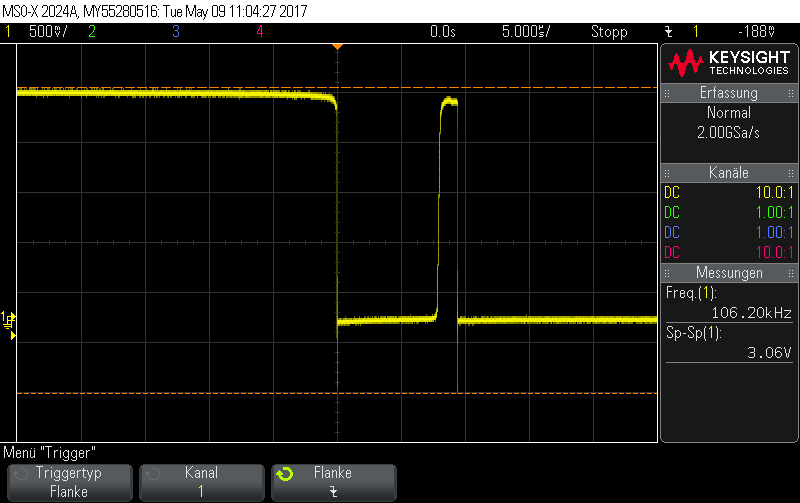
\includegraphics[width=0.49\textwidth]{Images/prellen1}} 
	\subfigure[Prellvorgang von ca $8ns$]{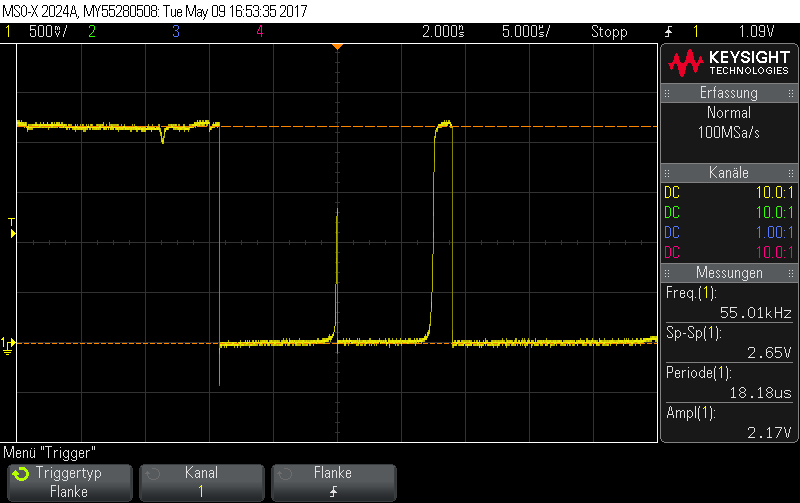
\includegraphics[width=0.49\textwidth]{Images/prellen2}} 
	%\caption{Titel unterm gesamten Bild}
	\subfigure[Prellvorgang von ca $6us$]{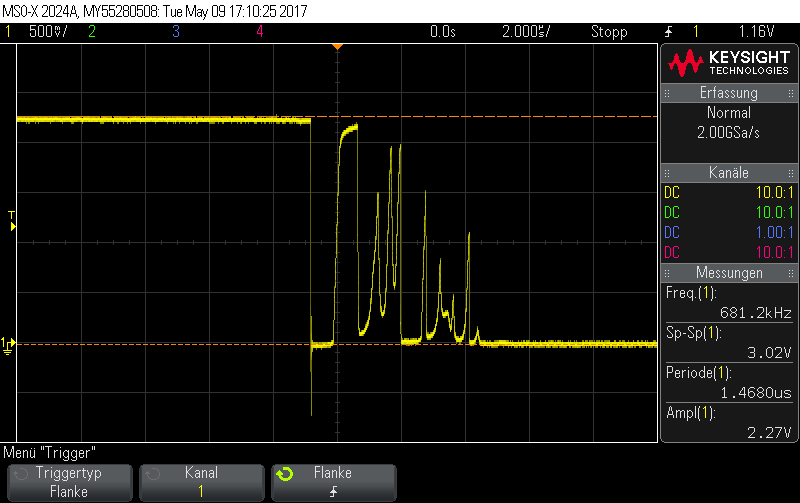
\includegraphics[width=0.49\textwidth]{Images/prellen3}} 
	\subfigure[Prellvorgang von ca $150us$]{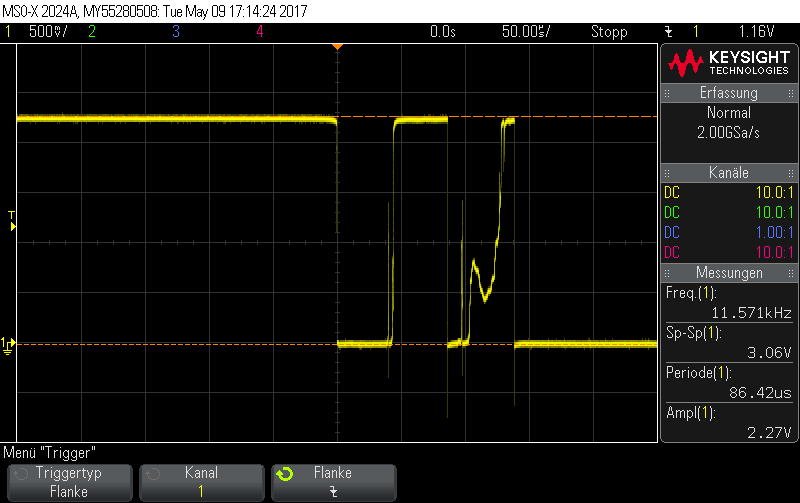
\includegraphics[width=0.49\textwidth]{Images/prellen4}} 
	%\caption{Titel unterm gesamten Bild} 
	\subfigure[Prellvorgang von ca $35us$]{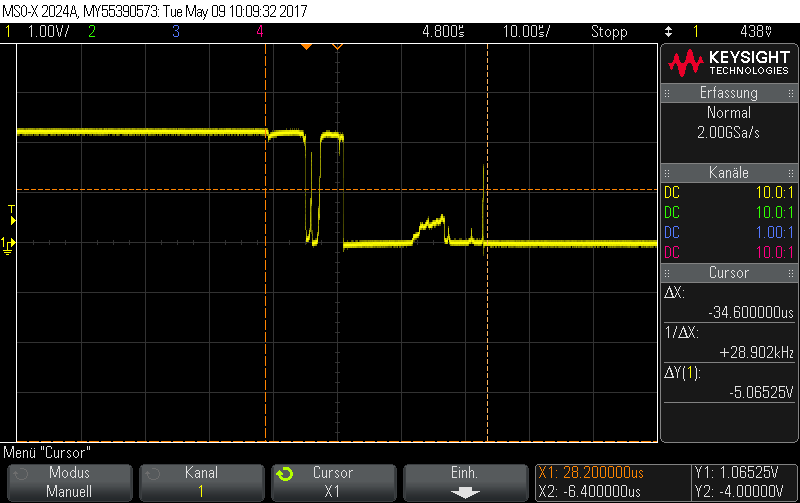
\includegraphics[width=0.49\textwidth]{Images/prellen5}} 
	\subfigure[Prellvorgang von ca $250us$]{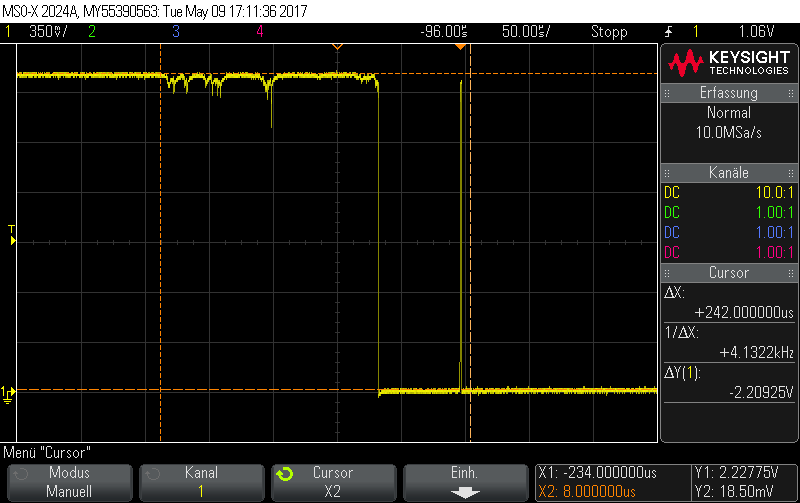
\includegraphics[width=0.49\textwidth]{Images/prellen6}} 
	\caption{Mehrere Prellvorgänge (entnommen aus Moodle)}
	\label{image:prellen}
\end{figure}

\newpage
\begin{figure}[h!]
	\centering
	\subfigure[Zeitliches Verhalten beim Prellen]{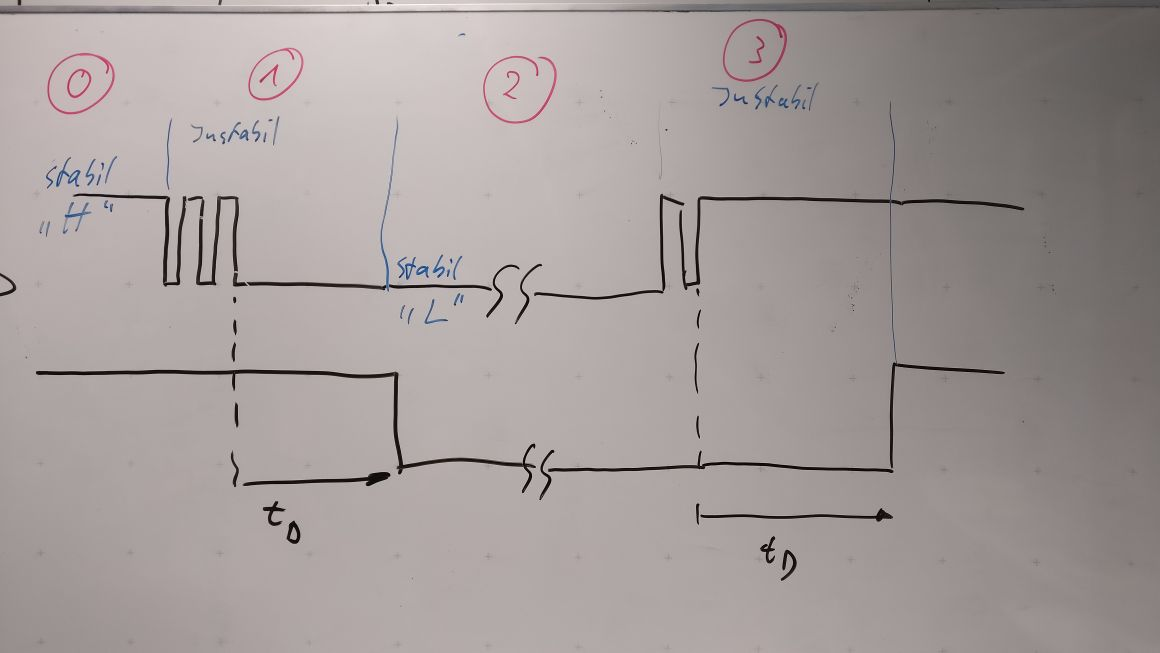
\includegraphics[width=\textwidth]{Images/statemachine2}} 
	\subfigure[Zustandsautomat]{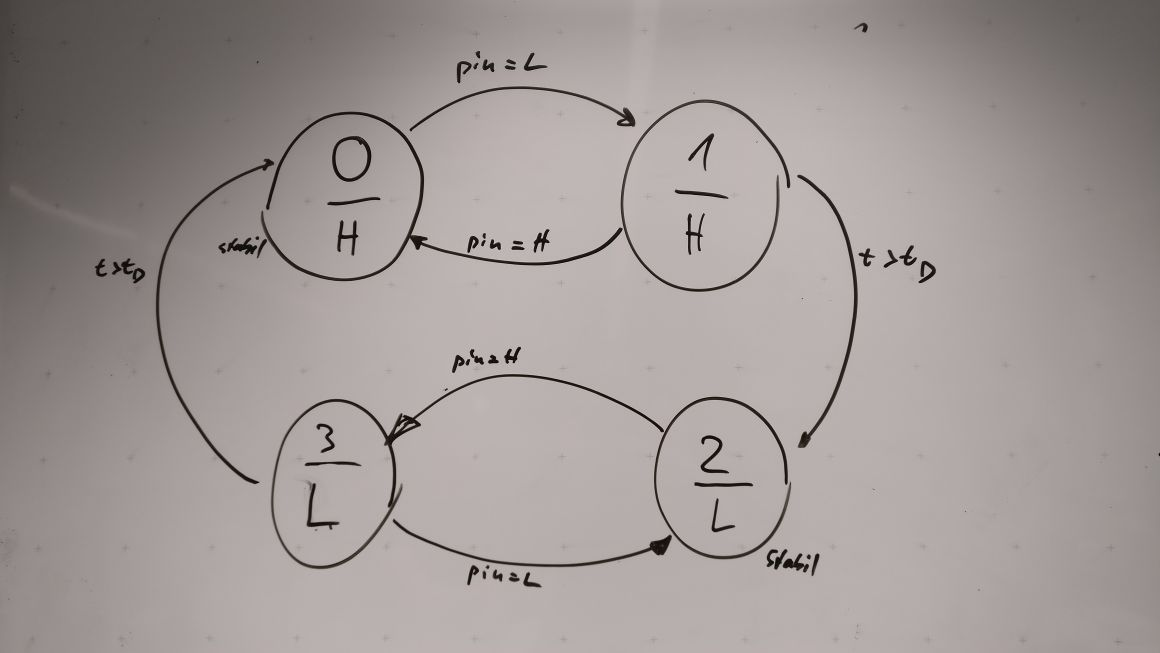
\includegraphics[width=\textwidth]{Images/statemachine}} 
	\caption[NonBlockingCode]{Skizzen zu der Funktion isPressed()}
	\label{image:statemachineispressed}
\end{figure}
\newpage